% ==============================================================================
% RESULTADOS
% ==============================================================================
% Instrucciones de la plantilla:
% - Por cada una de las actividades, describir detalladamente los resultados
%   alcanzados, tanto de las solicitadas, como de los experimentos.
% - Incluir capturas de pantalla debidamente tituladas y referenciadas en el texto.
% - REGLA: No se aceptarán solo capturas de pantalla; deben estar explicadas.
% - Analizar ventajas y desventajas de la metodología aplicada.
% ==============================================================================

\section{Resultados}

Las capturas de OpenGL de esta sección se tomaron del programa compilado con la configuración \texttt{Debug|x64}, a $1024 \times 768$.

% ------------------------------------------------------------------------------
\subsection{Resultados de la actividad: escena con diez fuentes de iluminación}
La Figura \ref{fig:res_diez} muestra la escena final con las diez fuentes encendidas, con la configuración de la Tabla \ref{tab:luces} y potencia de 30. Desde la cámara inicial se ven ocho marcadores, porque el techo tapa las dos fuentes de atrás. La casa y las cercas conservan sus texturas y nada se satura: la suma ambiental queda entre 0.61 y 0.67 en cada canal (Experimento 8).

\begin{figure}[H]
    \centering
    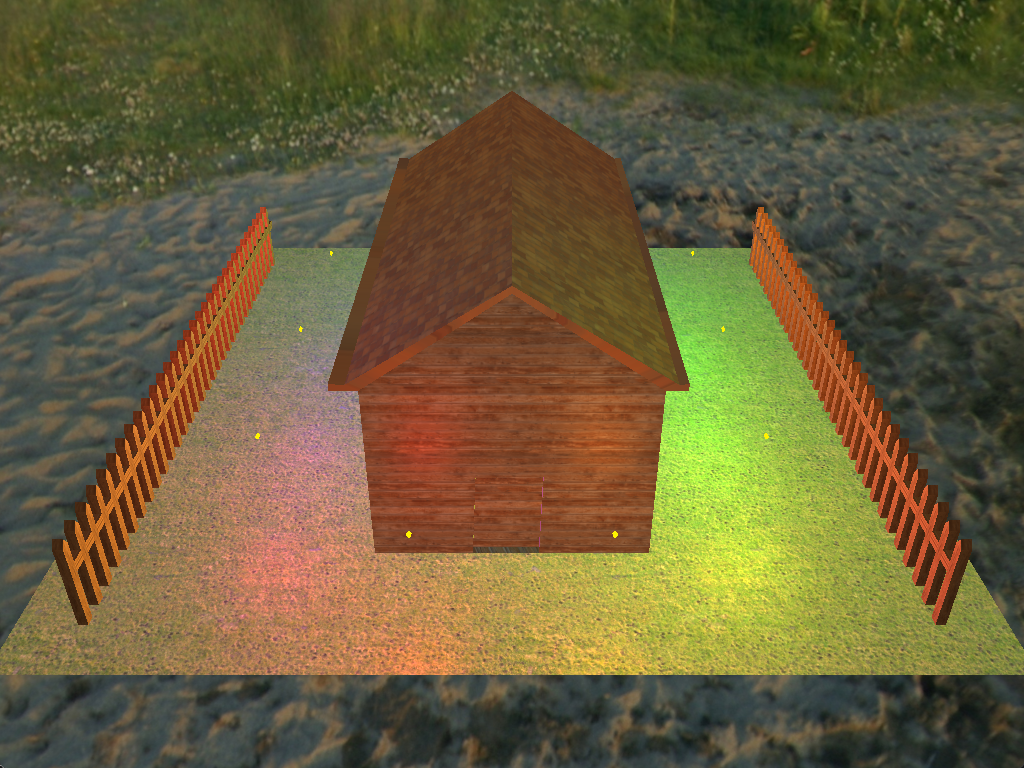
\includegraphics[width=0.75\textwidth]{Imagenes/Luces10/01_diez_luces.png}
    \caption{Resultado final: la casa iluminada por las diez fuentes de color.}
    \label{fig:res_diez}
\end{figure}

Los colores de las diez fuentes suman casi blanco (1.00, 0.98 y 0.92), pero la escena no queda de un solo color. La componente difusa y la especular dependen de la dirección a cada fuente, así que en cada zona pesan más las fuentes cercanas. El costado derecho del terreno se ve verde y amarillo por las fuentes 3, 4 y 5, el izquierdo se ve rosado y violeta por las fuentes 9 y 10, y la pared frontal tiene una mancha roja de la fuente 1. Las manchas brillantes del terreno son reflejos especulares: están donde el reflejo de cada fuente apunta a la cámara y se mueven al girarla, mientras que el resto del color se queda igual.

Para la Figura \ref{fig:res_superior} colocamos la cámara en $(0, 30, 0)$ mirando hacia abajo. Se ven los diez marcadores (dos al frente, abajo en la imagen, tres en cada costado y dos atrás), cada uno con un brillo de su color sobre el pasto. Los brillos de las fuentes de atrás se notan menos que los de los costados porque el reflejo especular depende de la posición de la cámara.

\begin{figure}[H]
    \centering
    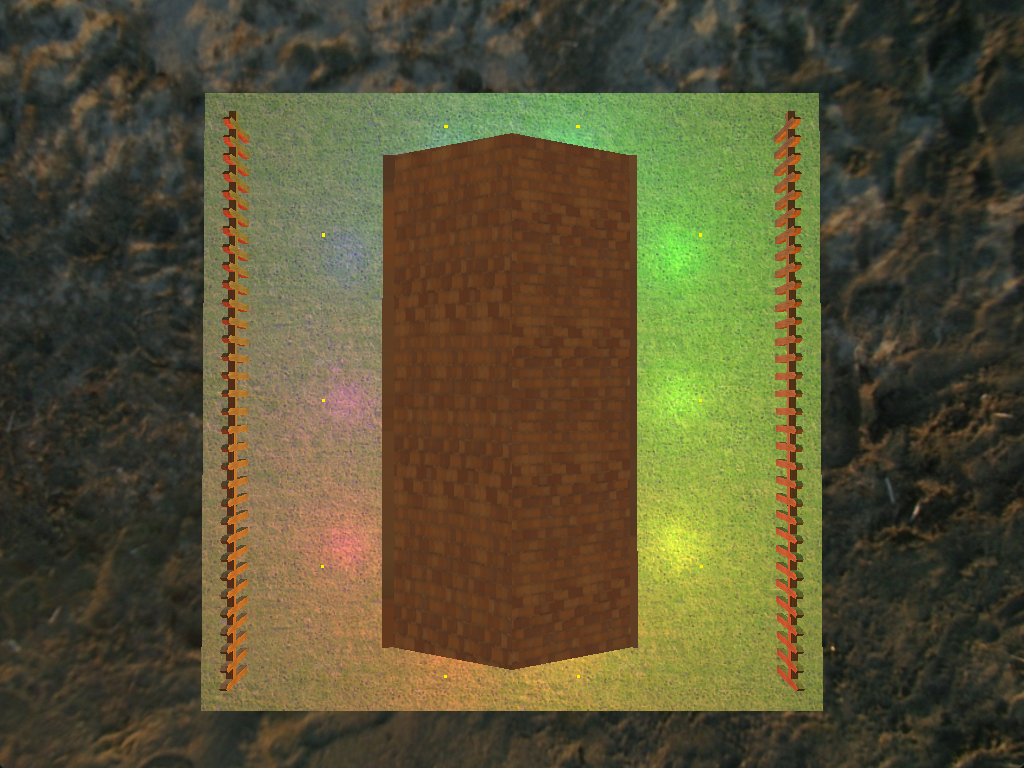
\includegraphics[width=0.75\textwidth]{Imagenes/Luces10/05_vista_superior.png}
    \caption{Vista superior de la escena: los diez marcadores de luz rodean la casa entre las paredes y la cerca.}
    \label{fig:res_superior}
\end{figure}

Las teclas numéricas apagan cualquier combinación de fuentes mientras corre el programa (Figuras \ref{fig:exp_una} a \ref{fig:exp_frias}). En el laboratorio, para ver el efecto de una fuente sola había que comentar líneas y volver a compilar.

\subsubsection{Análisis de ventajas y desventajas}
\begin{itemize}
    \item \textbf{Ventajas:} El \textit{shader} ya recibía un arreglo de fuentes, así que pasar de cuatro a diez solo requirió cambios en el \texttt{main}. Con las posiciones y los colores en dos arreglos, la configuración se cambia editando una tabla, y el teclado permite estudiar cada fuente sin recompilar. Como cada fuente tiene su propio color, en la imagen se distingue qué aporta cada una.
    \item \textbf{Desventajas:} Cada fragmento evalúa las diez fuentes aunque la mayoría aporte poco, así que el costo del \textit{fragment shader} crece con cada fuente. El límite de 10 está fijo en \texttt{MAX\_LIGHTS} y una fuente más exigiría modificar el \textit{shader}. Como la atenuación usa una distancia fija, todas las fuentes iluminan toda la escena con la misma intensidad, y la suma ambiental obliga a bajar la potencia conforme se agregan fuentes. El modelo tampoco calcula sombras, y la luz atraviesa la casa (Figura \ref{fig:exp_una}).
\end{itemize}

% ------------------------------------------------------------------------------
\subsection{Resultados de las pruebas del laboratorio}
En el laboratorio comprobamos que las fuentes de color se suman canal por canal: con una luz roja, una verde y una azul en la misma proporción, la casa se ve gris (Experimento 1). Con la textura, la luz solo tiñe la madera y el pasto. En la esfera, cada lado toma el color de la fuente que tiene enfrente, y al bajar la potencia o subir el exponente especular los brillos se separan y se hacen más pequeños. Los coeficientes de la tabla de materiales bastaron para reproducir la esmeralda y el rubí. En el programa de Fresnel, el índice de refracción determinó cuánto se deforma el fondo y \texttt{\_Bias} la proporción entre reflejo y refracción; con un valor de 1 la esfera se volvió un espejo.
\subsection{Resultados de la Actividad 2}
% Describir resultados y capturas para la Actividad 2:
\textit{Describir detalladamente los resultados obtenidos en la segunda actividad y referenciar sus figuras correspondientes...}

\subsection{Resultados de la Actividad 3}
\label{sec:act3_resultados}

Logramos visualizar el toroide exportado desde Blender en un programa independiente, con su textura de tablero y una fuente de luz blanca. El resultado permite cambiar la repetición de la imagen sin modificar la malla y activar o desactivar el cálculo de Phong. La superficie se muestra cerrada y el patrón recorre tanto la parte exterior como la interior del anillo.

\subsubsection{Efecto de la repetición UV}

En la Figura \ref{fig:act3_comparacion_uv} se observa que la repetición $1\times1$ produce cuadros grandes, mientras que $4\times4$ genera un patrón más denso. La silueta y la posición del toroide permanecen iguales, por lo que la diferencia corresponde al muestreo de la textura y no a un aumento de polígonos. Cerca de la parte interior los cuadros se ven más pequeños por la parametrización y la perspectiva de la superficie.

\begin{figure}[H]
    \centering
    \begin{minipage}[t]{0.48\textwidth}
        \centering
        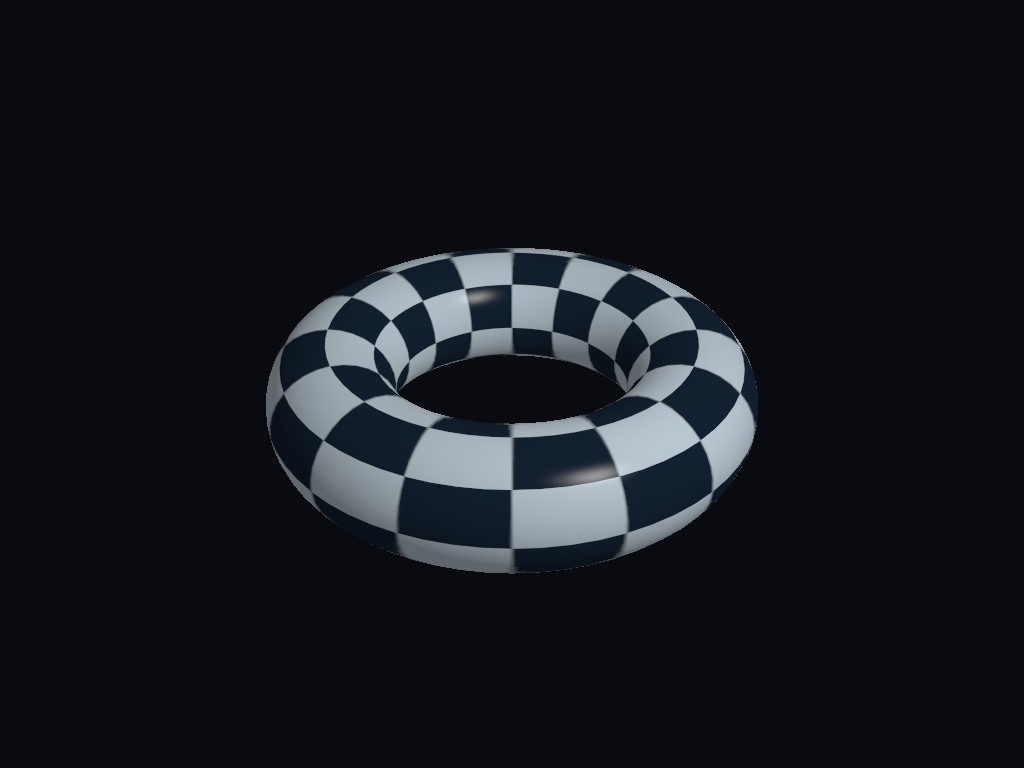
\includegraphics[width=\linewidth]{Imagenes/E3/act3_phong_1x1.png}
        \par\small (a) Repetición $1\times1$.
    \end{minipage}\hfill
    \begin{minipage}[t]{0.48\textwidth}
        \centering
        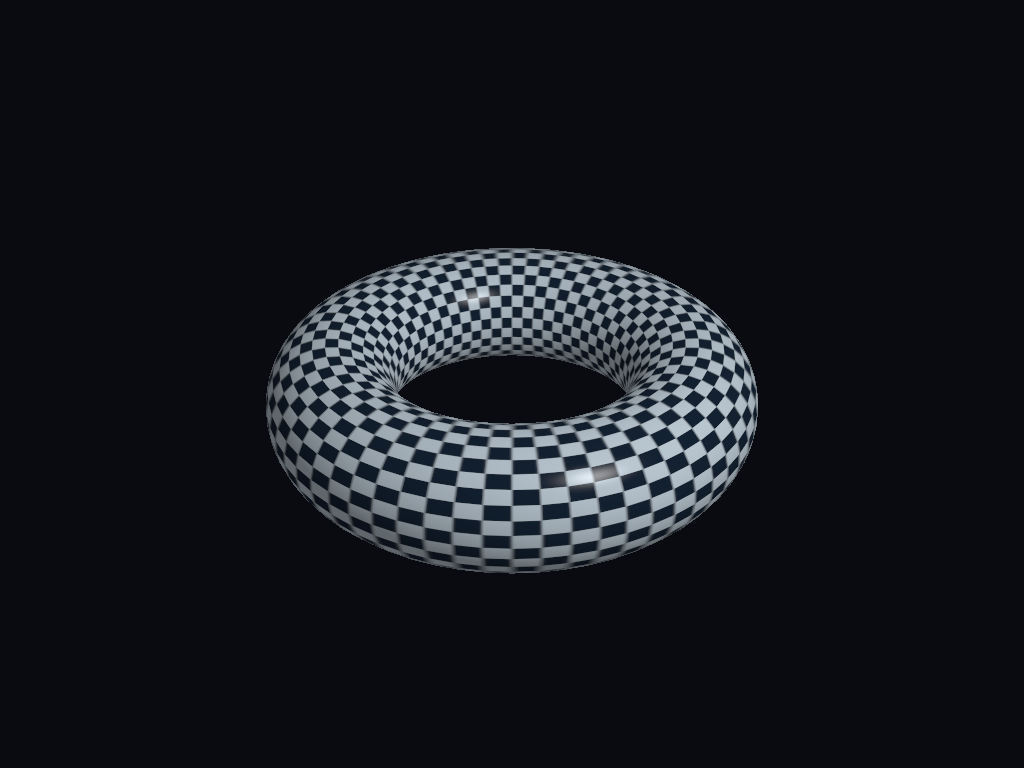
\includegraphics[width=\linewidth]{Imagenes/E3/act3_phong_4x4.png}
        \par\small (b) Repetición $4\times4$.
    \end{minipage}
    \caption{Comparación de la repetición de textura con la misma geometría, cámara e iluminación Phong.}
    \label{fig:act3_comparacion_uv}
\end{figure}

\subsubsection{Efecto de la iluminación Phong}

La Figura \ref{fig:act3_comparacion_luz} muestra que, sin iluminación, los cuadros conservan un color prácticamente uniforme y la sensación de volumen depende principalmente de la silueta y de la perspectiva del patrón. Al activar Phong aparecen transiciones de intensidad y pequeños brillos que hacen más evidente la curvatura del tubo. La textura sigue siendo la misma; lo que cambia es la respuesta de la superficie frente a la luz y a la posición de la cámara.

\begin{figure}[H]
    \centering
    \begin{minipage}[t]{0.48\textwidth}
        \centering
        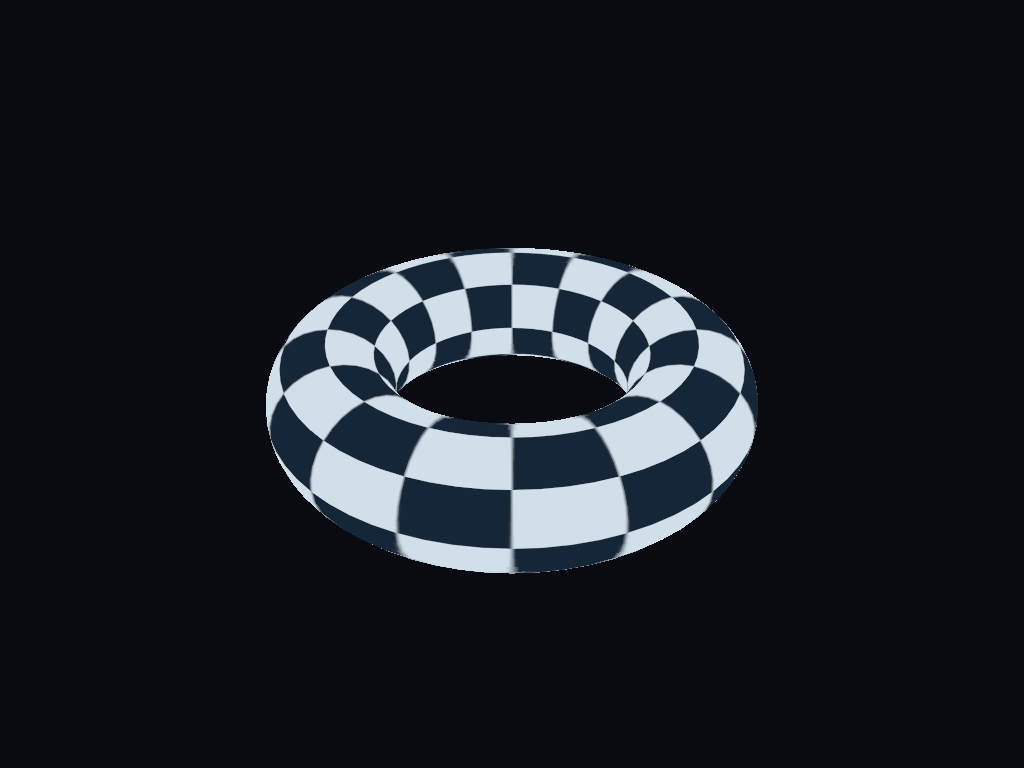
\includegraphics[width=\linewidth]{Imagenes/E3/act3_sin_luz_1x1.png}
        \par\small (a) Textura sin iluminación.
    \end{minipage}\hfill
    \begin{minipage}[t]{0.48\textwidth}
        \centering
        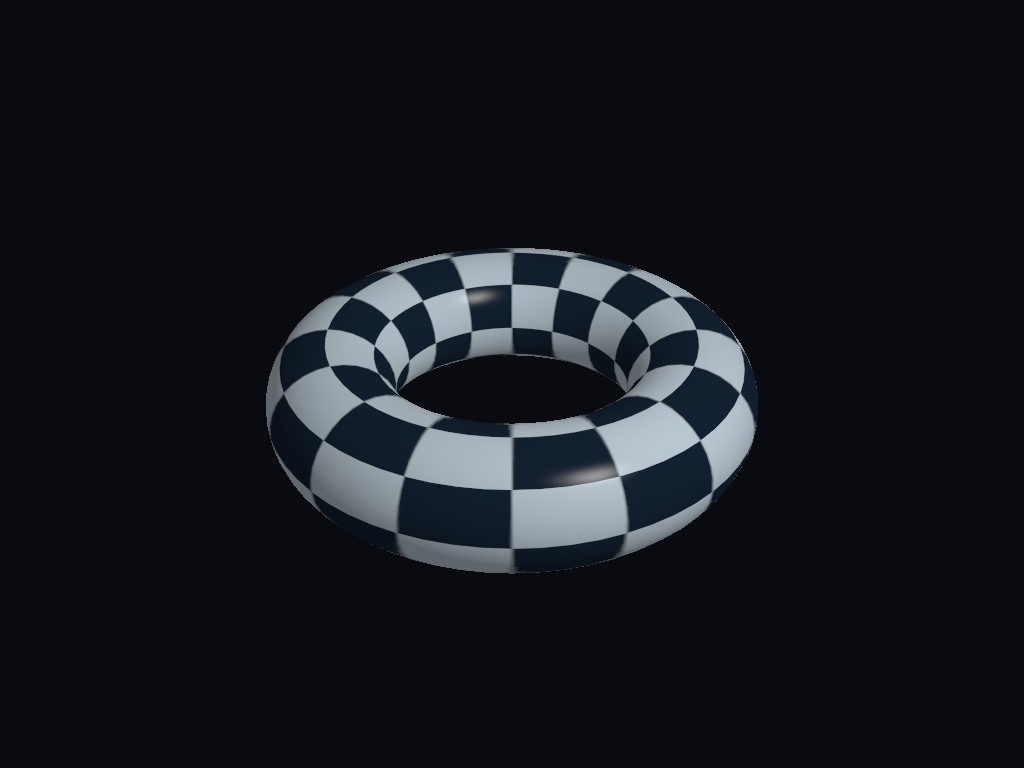
\includegraphics[width=\linewidth]{Imagenes/E3/act3_phong_1x1.png}
        \par\small (b) Textura con Phong.
    \end{minipage}
    \caption{Cambio de apariencia al activar Phong, manteniendo la repetición de textura en $1\times1$.}
    \label{fig:act3_comparacion_luz}
\end{figure}

También se obtuvo la vista sin iluminación con repetición $4\times4$, mostrada en la Figura \ref{fig:act3_sin_luz_4x4}. Esta imagen confirma que el aumento en la cantidad de cuadros no depende de Phong: el patrón cambia incluso cuando se desactiva la iluminación.

\begin{figure}[H]
    \centering
    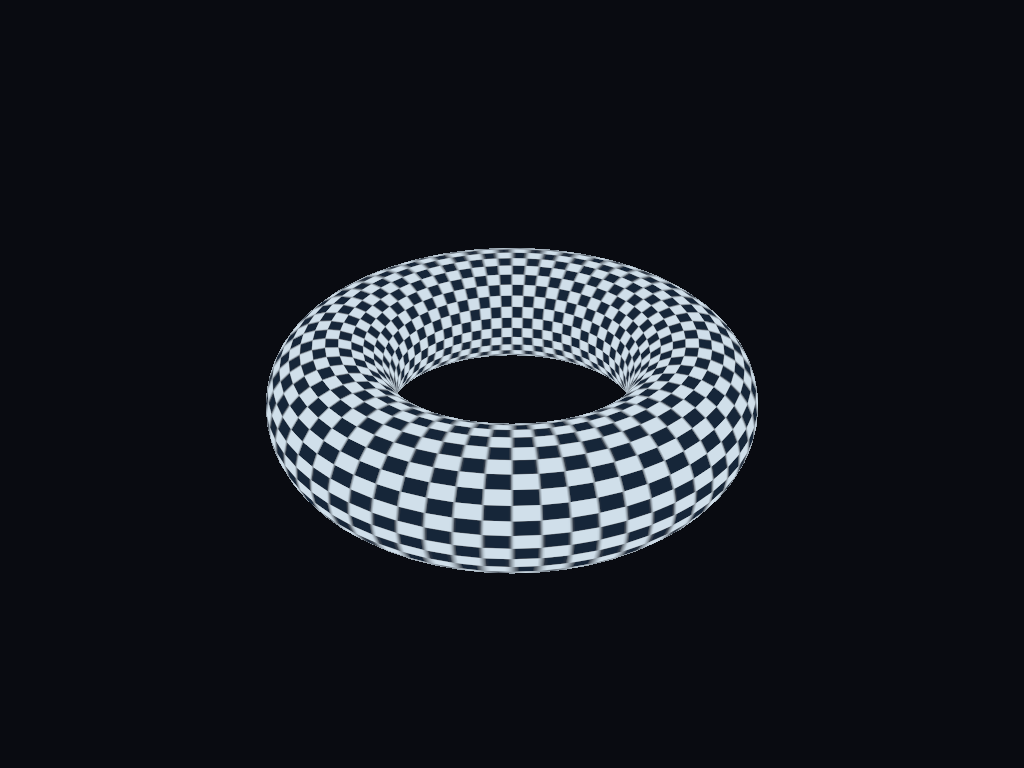
\includegraphics[width=0.48\textwidth]{Imagenes/E3/act3_sin_luz_4x4.png}
    \caption{Textura repetida $4\times4$ sin cálculo de iluminación.}
    \label{fig:act3_sin_luz_4x4}
\end{figure}

\subsubsection{Verificación del modelo y del programa}

La malla de Blender contiene 2048 vértices, mientras que la importada utiliza 2145. Esta diferencia se debe a que algunos puntos de la costura necesitan registros separados para conservar sus coordenadas UV, aunque compartan posición. En ambos casos se mantienen 4096 triángulos, por lo que no se agregó detalle geométrico durante la carga.

Las cuatro pruebas automatizadas principales terminaron correctamente: verificación de recursos, lectura desde otro directorio, rechazo de argumentos inválidos y prueba del pipeline OpenGL. Esta última incluyó las capturas, las imágenes RGB y RGBA y los errores controlados descritos en la sección de experimentos.

\subsubsection{Ventajas y limitaciones}

\begin{itemize}
    \item \textbf{Ventajas:} el modelo y la textura son recursos separados que pueden reutilizarse; el tablero facilita revisar las UV; y la comparación con la misma cámara permite identificar el efecto de la iluminación sin confundirlo con un cambio de geometría.
    \item \textbf{Limitaciones:} Phong proporciona iluminación local, pero el programa no calcula sombras proyectadas, reflejos del entorno ni refracción. La distribución de cuadros no tiene el mismo tamaño físico en todo el toroide. Además, la textura utilizada es una prueba del pipeline y no representa todavía los materiales de mármol, madera, oro, bronce, cobre y cristal solicitados para completar la actividad del manual.
\end{itemize}

\subsection{Resultados de la Actividad 4}
\label{sec:act4_resultados}

La Figura \ref{fig:act4_resultado} muestra los seis materiales con la misma iluminación. Arriba están el mármol, la madera y el oro; abajo, el bronce, el cobre y el cristal.

\begin{figure}[H]
    \centering
    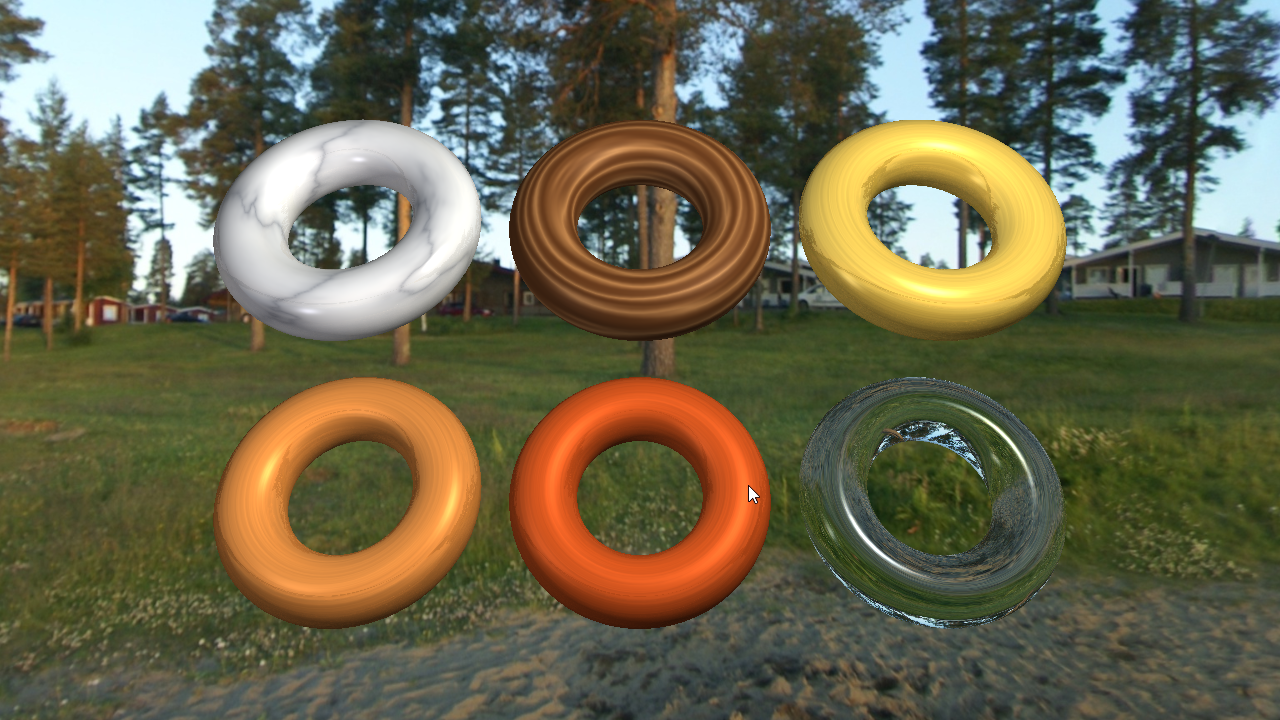
\includegraphics[width=0.95\textwidth]{Imagenes/E4/materiales_con_textura.png}
    \caption{Toroides de mármol, madera y oro (arriba) y de bronce, cobre y cristal (abajo).}
    \label{fig:act4_resultado}
\end{figure}

El mármol es el más claro y tiene el brillo más pequeño y definido ($q = 96$); las vetas siguen la curvatura del tubo y se ven bien en la parte interior. En la madera los anillos corren a lo largo del tubo y el brillo casi no aparece, que es lo que se espera de una madera sin barniz. Los metales se reconocen sobre todo por el color del reflejo. En el oro el brillo es más angosto que en el bronce y en el cobre, como corresponde a su exponente mayor (51.2 contra 25.6 y 12.8), y el rayado del metal cepillado solo se nota de cerca. El cristal es el único que no depende de Phong para verse: a través del tubo se ve el pasto deformado por la refracción, y en los bordes aparece el cielo reflejado, como predice la Ecuación \ref{eq:schlick}.

\subsubsection{Ventajas y limitaciones}

Con un solo shader y seis juegos de parámetros salen materiales muy distintos, y agregar otro es solo agregar una fila a la tabla. Pero el reflejo viene de un cubemap fijo: los toroides no se reflejan entre sí, y el cristal no muestra a los otros toroides detrás de él. Tampoco hay sombras. Los valores de mármol y madera los ajustamos a ojo y no salen de una medición.

\subsection{Resultados de las variaciones}
\label{sec:var_resultados}

\subsubsection{Actividad 1: fuentes en órbita}

Después de girar, las manchas de color cambiaron de lugar en el terreno y en la casa (Figura \ref{fig:var1}). Al inicio el rojo y el naranja quedaban al frente, a la izquierda, y el verde a la derecha. Después de la órbita el verde pasó al lado izquierdo y el rojo al derecho. La casa no se movió: el cambio de color viene solo de la nueva posición de cada fuente, porque $\mathbf{l}_i$ en la Ecuación \ref{eq:phong_multi} depende de ella.

\begin{figure}[H]
    \centering
    \begin{minipage}[t]{0.48\textwidth}
        \centering
        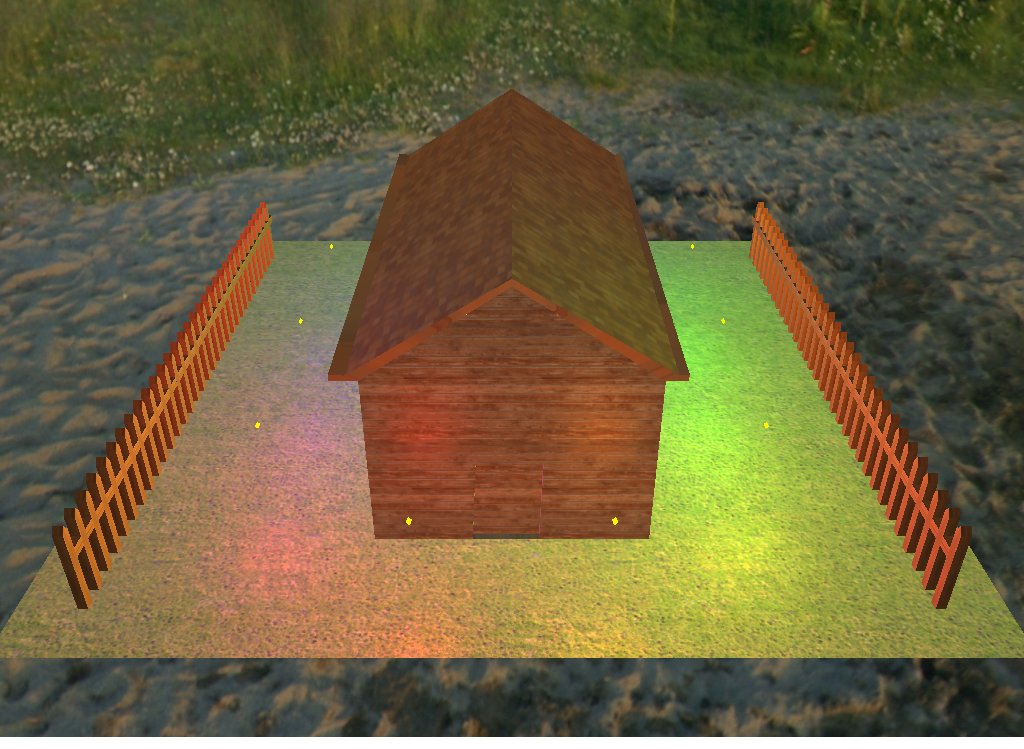
\includegraphics[width=\linewidth]{Imagenes/Variaciones/v1_inicial.png}
        \par\small (a) Posición inicial.
    \end{minipage}\hfill
    \begin{minipage}[t]{0.48\textwidth}
        \centering
        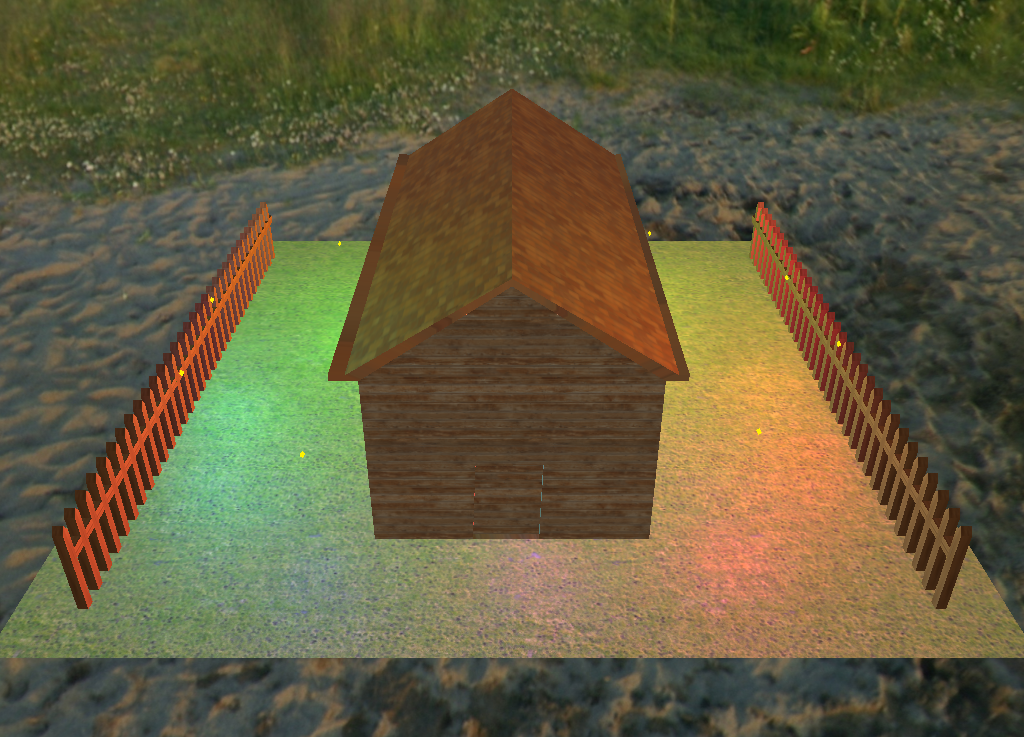
\includegraphics[width=\linewidth]{Imagenes/Variaciones/v1_girada.png}
        \par\small (b) Después de la órbita.
    \end{minipage}
    \caption{Variación de la actividad 1: las diez fuentes antes y después de girar alrededor de la casa.}
    \label{fig:var1}
\end{figure}

\subsubsection{Actividad 2}

Con los plásticos opacos, la esfera roja tiene dos brillos blancos pequeños, uno por cada fuente, y la casa no tiene ninguno porque su especular es casi cero. Esa diferencia es lo que separa un plástico de un material mate. Con transparencia de 0.45 se ven la pared de la casa y el pasto a través de la esfera y de la mesa (Figura \ref{fig:var2}). En la esfera también se alcanza a ver su cara trasera, más clara, porque el programa no ordena los triángulos del mismo objeto.

\begin{figure}[H]
    \centering
    \begin{minipage}[t]{0.48\textwidth}
        \centering
        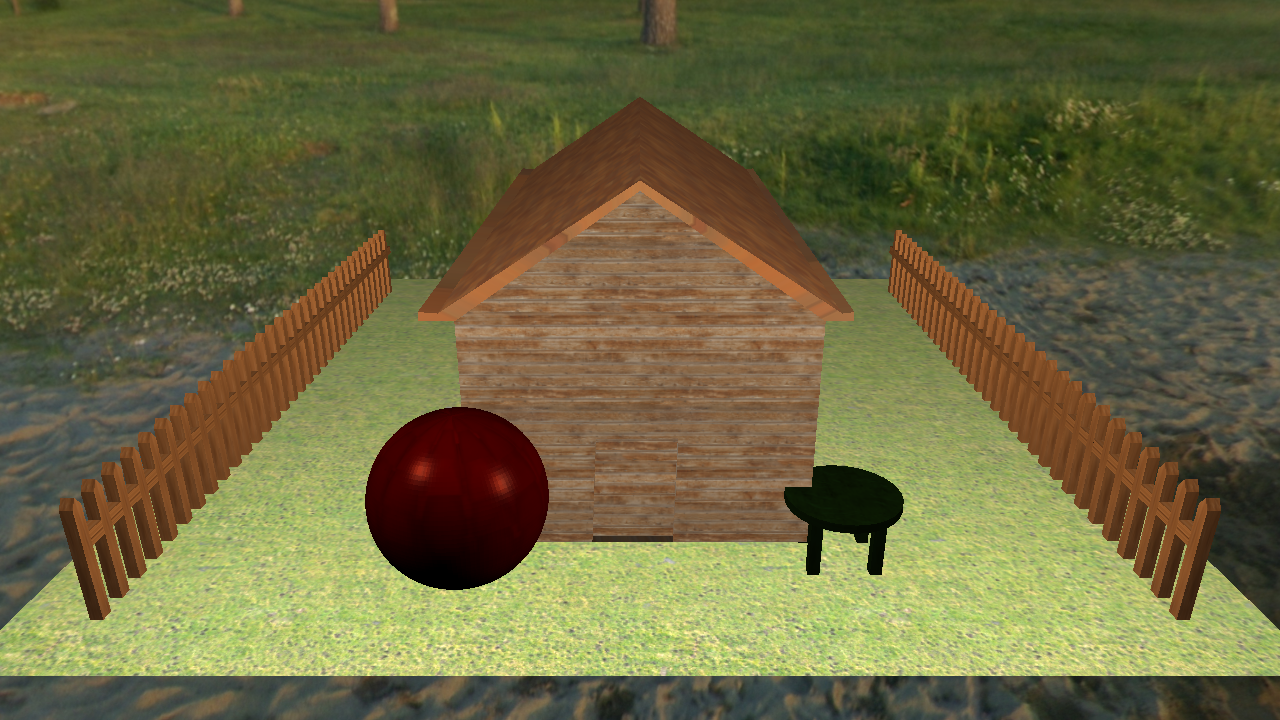
\includegraphics[width=\linewidth]{Imagenes/Variaciones/v2_opacos.png}
        \par\small (a) Plásticos opacos.
    \end{minipage}\hfill
    \begin{minipage}[t]{0.48\textwidth}
        \centering
        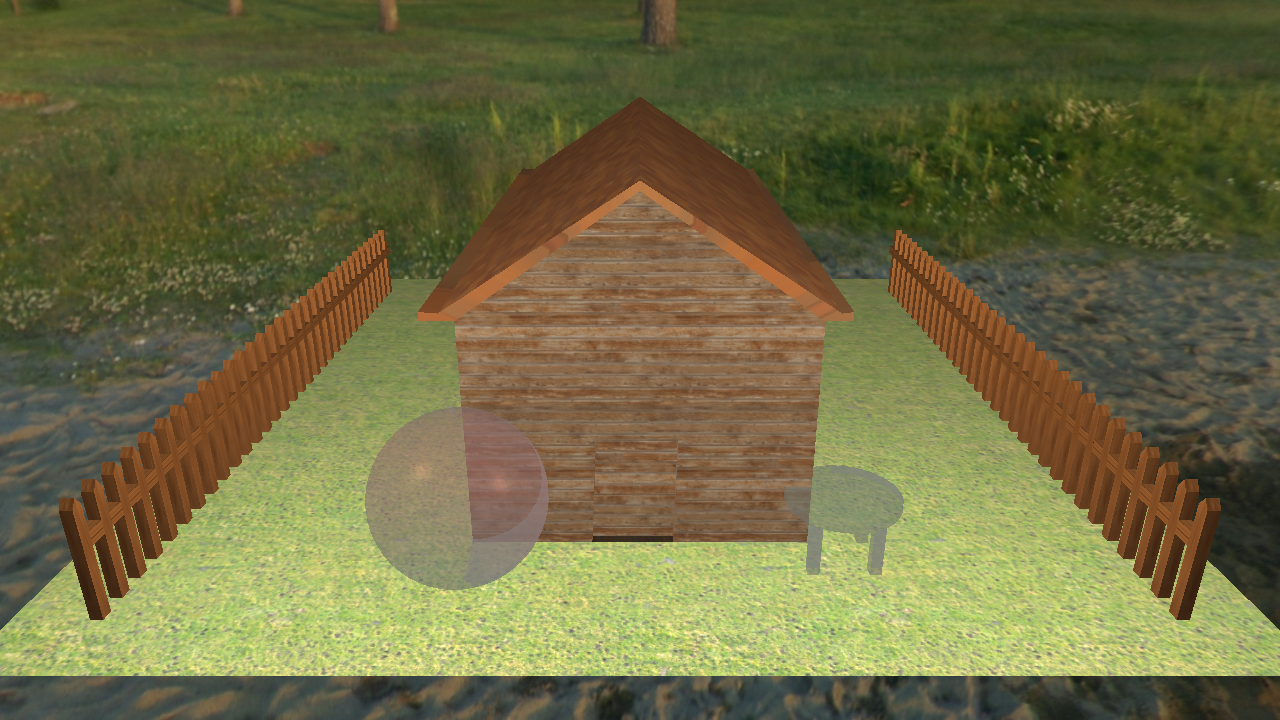
\includegraphics[width=\linewidth]{Imagenes/Variaciones/v2_translucidos.png}
        \par\small (b) Transparencia 0.45.
    \end{minipage}
    \caption{Variación de la actividad 2: casa opaca, esfera de plástico rojo y mesa de plástico verde.}
    \label{fig:var2}
\end{figure}

\subsubsection{Actividad 3: filtrado de textura}

Con \texttt{GL\_NEAREST} cada píxel toma el color de un solo texel. En la parte de atrás del anillo los cuadros miden menos de un píxel y aparecen patrones de moiré y bordes dentados en la silueta del tablero. Con mipmaps esa zona se ve gris parejo, porque OpenGL usa una versión reducida de la imagen que ya promedia el blanco y el negro (Figura \ref{fig:var3}). Al frente, donde los cuadros son grandes, los dos filtros se ven casi iguales. El costo de los mipmaps es la memoria extra (alrededor de un tercio más) y que de lejos la imagen pierde nitidez.

\begin{figure}[H]
    \centering
    \begin{minipage}[t]{0.48\textwidth}
        \centering
        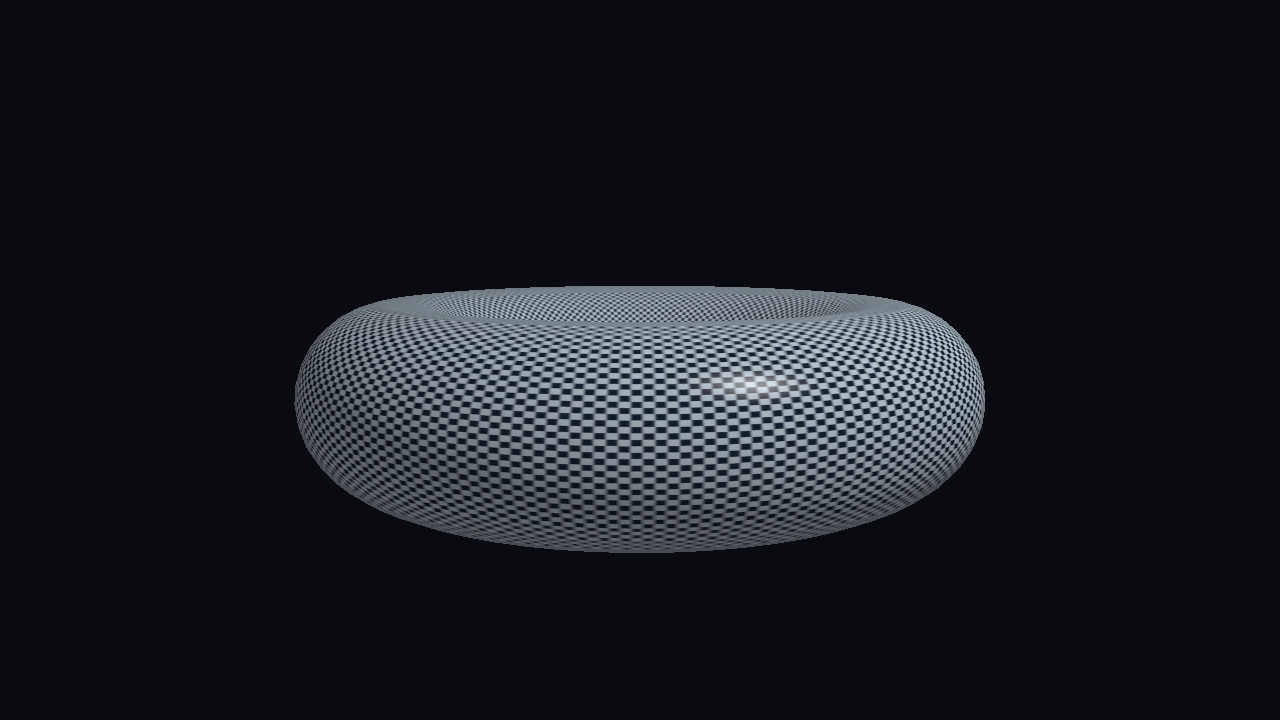
\includegraphics[width=\linewidth]{Imagenes/Variaciones/v3_mipmaps.png}
        \par\small (a) Mipmaps, filtrado trilineal.
    \end{minipage}\hfill
    \begin{minipage}[t]{0.48\textwidth}
        \centering
        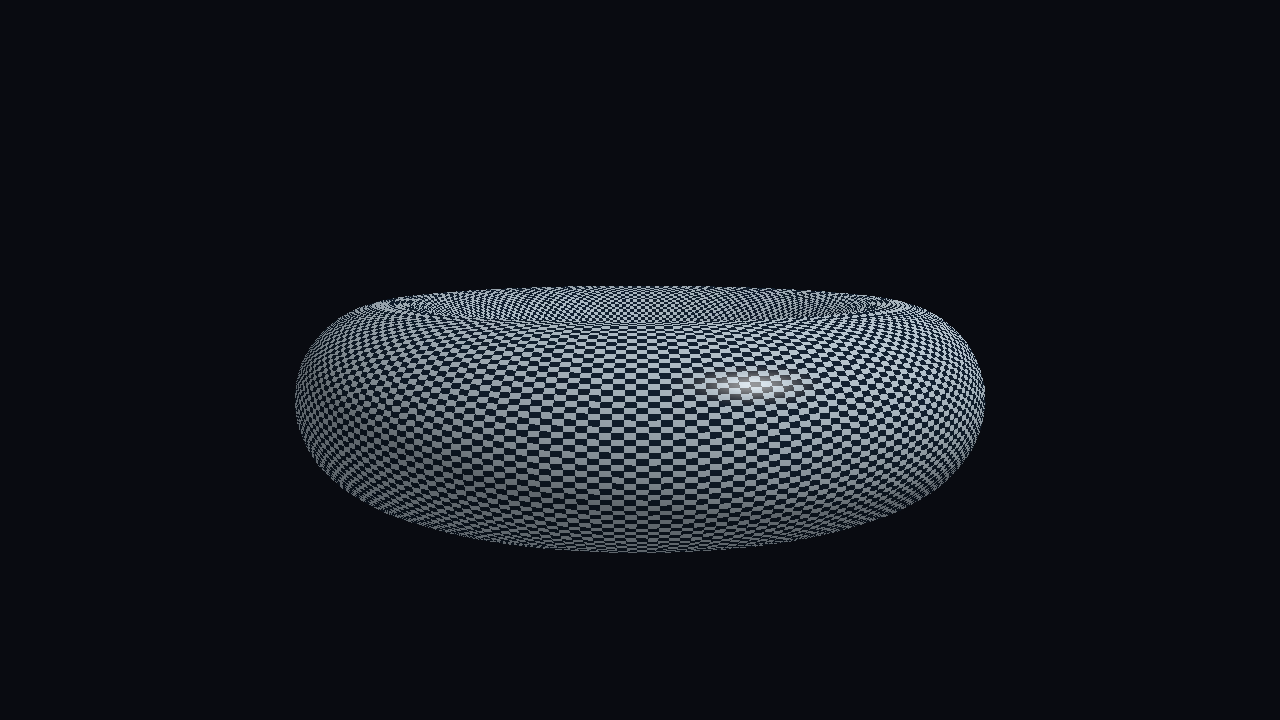
\includegraphics[width=\linewidth]{Imagenes/Variaciones/v3_nearest.png}
        \par\small (b) \texttt{GL\_NEAREST}.
    \end{minipage}
    \caption{Variación de la actividad 3: el tablero repetido $16\times16$ con los dos filtros.}
    \label{fig:var3}
\end{figure}

\subsubsection{Actividad 4: materiales sin textura}

Sin textura, el mármol y la madera quedaron como dos toroides blancos casi iguales (Figura \ref{fig:var4}); solo se diferencian en el brillo, que en la madera casi no existe. Los metales cambiaron poco porque su color viene de los coeficientes de la tabla y del reflejo; solo perdieron el rayado. El cristal quedó igual porque no usa textura. Con esto se ve qué parte de cada material sale de la imagen y qué parte de los parámetros de iluminación.

\begin{figure}[H]
    \centering
    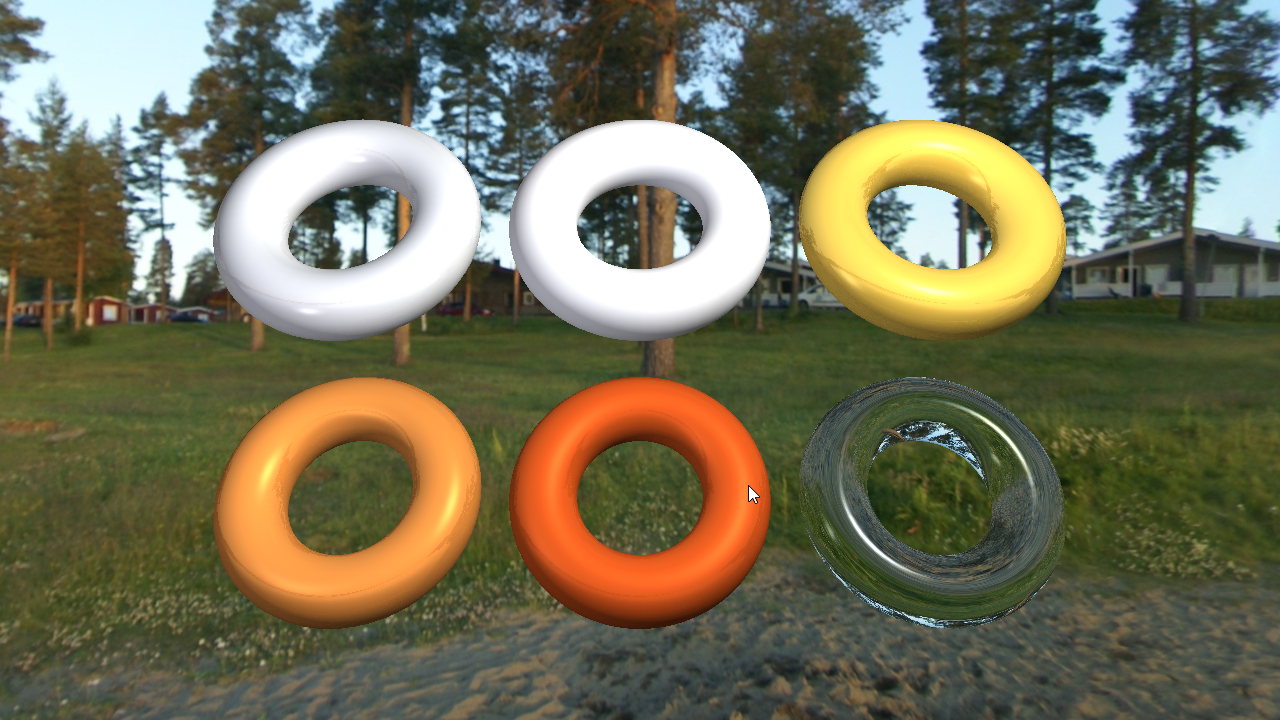
\includegraphics[width=0.95\textwidth]{Imagenes/E4/materiales_sin_textura.png}
    \caption{Variación de la actividad 4: los mismos materiales sin la información de textura.}
    \label{fig:var4}
\end{figure}
